\section{Diagramas de Clases de Diseño}

El diagrama de clases de diseño se abstrae de las relaciones entre los objetos detallados en los diagramas de secuencia y los mensajes (invocaciones a objetos) con los que se comunicaban.

Los diagramas de clases se separaron en clases de Cliente y de Administrador, en la figura~\ref{fig:DiaramaCasoDeDisenio} mostramos la sección de administrar cliente.

\begin{figure}[H]
    \centering
    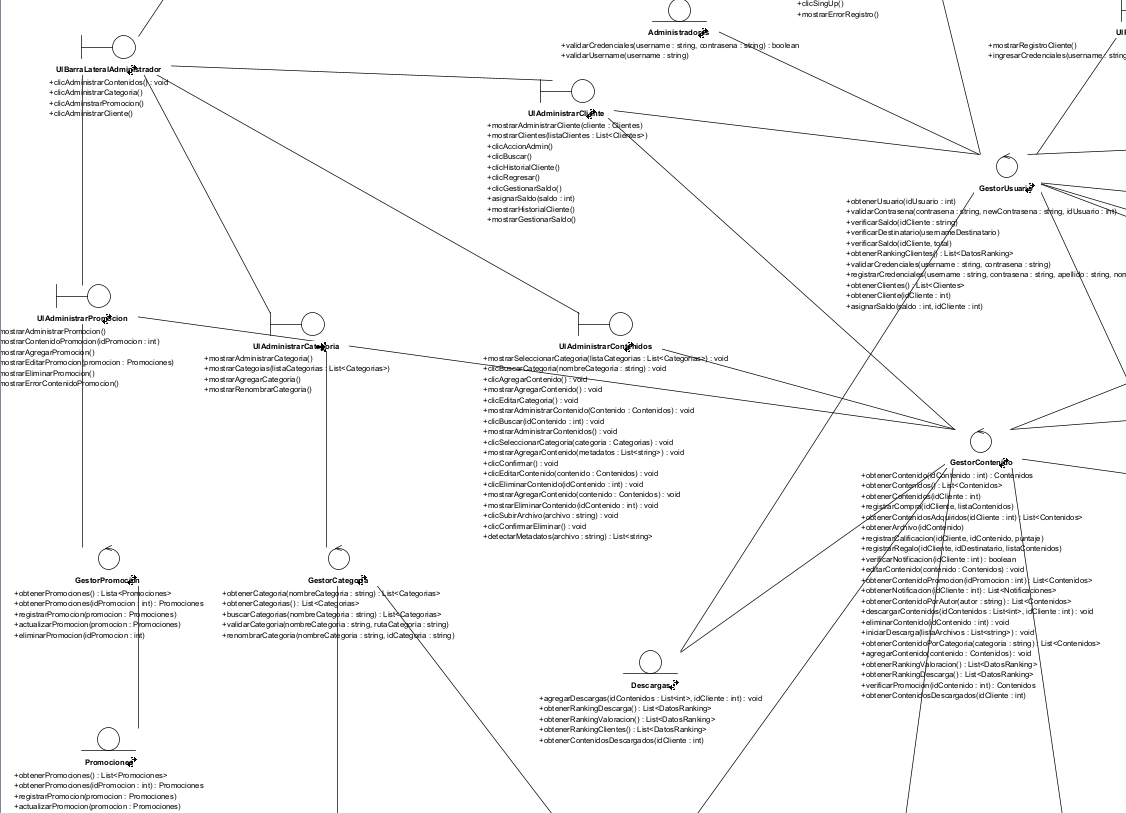
\includegraphics[width=0.9\textwidth]{Media/4_Disenio/DCAdmin.png}
    \caption{Diagrama de clases de diseño la sección Administrar Cliente} 
    \label{fig:DiaramaCasoDeDisenio}
\end{figure}

\textbf{Archivo:} \texttt{Diagramas de Clases de Diseño} \\
\textbf{Link de acceso:} \linkDiagramaClases \\

\textbf{Pasos de ejecución:}
\begin{enumerate}
    \item Ingresar al repositorio en GitHub usando el link proporcionado y descargar el archivo QCM.vpp
    \item Abrir el archivo descargado en la herramienta Visual Paradigm.
    \item En la pestaña Diagram Navigator abrir UML Diagrams
    \item Abrir Class Diagram y seleccionar Sistema Portal de Descargas Class Diagram.
\end{enumerate}

\subsection{ Diccionario de Diagramas de Clases de Diseño}
El diccionario de clases de diseño está compuesto por el nombre de la clase, su identificador, sus atributos y métodos con sus respectivas descripciones, tipo de dato de retorno y visibilidad, así como se muestra en la tabla~\ref{tab:diccionarioClasesMK038}. 

% ==== MK-038 ====
%%%%%%%%%%%%%%%%%%%%%%%%%%%%%%%%%%%%%%%%%%%%%%%%%
\renewcommand{\arraystretch}{1.3}
\begin{longtable}{|p{3.5cm}|p{2cm}|p{2cm}|p{6cm}|}
\caption{Diccionario de MK-038 UIAdministrarCliente}
\label{tab:diccionarioClasesMK038} \\
    \hline
    \multicolumn{2}{|p{5.5cm}|}{\textbf{Nombre:}}    & \multicolumn{2}{p{6cm}|}{UIAdministrarCliente} \\
    \hline
    \multicolumn{2}{|p{5.5cm}|}{\textbf{ID:}}        & \multicolumn{2}{p{6cm}|}{MK-038} \\
    \hline
    \multicolumn{2}{|p{5.5cm}|}{\textbf{Descripción:}} 
                                              & \multicolumn{2}{p{6cm}|}{Interfaz que permite al administrador visualizar, buscar y gestionar la información de los clientes registrados, incluyendo su historial y saldo.} \\
    \hline
    \endfirsthead

    \multicolumn{4}{c}{\textbf{continuación desde la página anterior}} \\
    \endhead

    \hline \multicolumn{4}{r}{{Continúa en la siguiente página}} \\
    \endfoot    

    \hline
    \endlastfoot

    \textbf{Atributo}    & \textbf{Tipo de datos} & \textbf{Visibilidad} & \textbf{Descripción} \\
    \hline
    - listaClientes & List\textless. datosCliente \textgreater & Privada & Lista de clientes obtenida desde la base de datos (BD-001), que se muestra en pantalla para su gestión. \\
    \hline

    \multicolumn{4}{|p{13.5cm}|}{\textbf{Métodos}} \\
    \hline
    \textbf{Método} & \textbf{Tipo de dato} & \textbf{Visibilidad} & \textbf{Descripción} \\
    \hline
    + mostrarAdministrarCliente() & void & Pública & Muestra la interfaz principal para la administración de clientes. \\
    \hline
    + mostrarClientes(clientes: List\textless datosCliente\textgreater) & void & Pública & Muestra los datos de los clientes en una tabla. \\
    \hline
    + clicGestionarSaldo() & void & Pública & Inicia la acción para modificar el saldo de un cliente seleccionado. \\
    \hline
    + refrescar() & void & Pública & Actualiza los datos mostrados en pantalla. \\
    \hline
    + clicVerHistorial() & void & Pública & Redirige a la vista donde se muestra el historial de contenidos descargados por el cliente. \\
    \hline
    + clicBuscar(idCliente: int) & void & Pública & Filtra la lista de clientes para mostrar solo el que coincide con el código ingresado. \\
    \hline
\end{longtable}

\textbf{Documento:}{Diccionario de Diagramas de Clases (PDF)} \\
\textbf{Link de acceso:} \linkDiccionarioClases \\


